\documentclass{beamer}


% Load essential packages
\usepackage{hyperref} % Only load once to avoid conflicts
\usepackage{stile}
\usepackage{subcaption}
\usepackage{tcolorbox}
\usepackage[font=scriptsize,skip=1pt]{caption}
\usepackage[T1]{fontenc}
\usepackage{csquotes}
\usepackage[backend=biber, style=authoryear, maxnames=3, minnames=1, abbreviate=false, date=long, url=false, isbn=false, doi=false]{biblatex}
\addbibresource{lecture1/bib.bib} % Ensure this matches your bibliography file name

\interfootnotelinepenalty=10000

\usepackage{latexsym, amsmath, xcolor, multicol, booktabs, calligra}
\usepackage{graphicx, pstricks, listings, stackengine}

% Hyperref setup
\hypersetup{
    hidelinks,
    colorlinks=true,
    linkcolor=black,
    citecolor=deepblue,
    urlcolor=black
}

% Font theme for Beamer
\usefonttheme[onlymath]{serif}

% Custom definitions
\def\cmd#1{\texttt{\color{red}\footnotesize $\backslash$#1}}
\def\env#1{\texttt{\color{blue}\footnotesize #1}}
\definecolor{deepblue}{rgb}{0,0,0.5}
\definecolor{deepred}{rgb}{0.6,0,0}
\definecolor{deepgreen}{rgb}{0,0.5,0}
\definecolor{halfgray}{gray}{0.55}

% Beamer color settings
\setbeamercolor{block title}{bg=blue!70!white, fg=white}
\setbeamercolor{block body}{bg=blue!10!halfgray, fg=white}
\setbeamercolor{section in head/foot}{fg=white}
\setbeamercolor{subsection in head/foot}{fg=white}
\setbeamercolor{title in head/foot}{fg=white}


% Listings settings for code highlighting
\lstset{
    basicstyle=\ttfamily\small,
    keywordstyle=\bfseries\color{deepblue},
    emphstyle=\ttfamily\color{deepred},
    stringstyle=\color{deepgreen},
    numbers=left,
    numberstyle=\small\color{halfgray},
    rulesepcolor=\color{red!20!green!20!blue!20},
    frame=shadowbox,
}

\author{Freya Rubel}
\title{Trade, Migration and Global Challenges}
\subtitle{Introduction to Globalization}
\institute{}
\date{20.10.2026}

\graphicspath{{lecture1/}}

\begin{document}

\begin{frame}
    \titlepage
\end{frame}

\begin{frame}
    \tableofcontents[sectionstyle=show, subsectionstyle=show/shaded/hide, subsubsectionstyle=show/shaded/hide]
\end{frame}

\section{Stylized Facts}

\begin{frame}{Definition}
    \textbf{What is Globalization?} \vspace{0.5cm} \\
    \pause
The IMF (International Monetary Fund) defines globalization as: “the increasing integration of economies around the world, particularly through the movement of \textbf{goods}, \textbf{services}, and \textbf{capital} across borders.”
\vspace{0.2cm}\\
\pause
The World Bank once summed up globalization as follows: “It might mean sitting in your living room in Estonia while communicating with a friend in Zimbabwe. It might mean taking a Bollywood dance class in London. Or it might be symbolized in eating Ecuadorian bananas in the European Union.”
\end{frame}

\begin{frame}{How Do We Measure Globalization?}
\small
\textbf{Why Measurement Matters:}
\begin{itemize}
    \item Is our world becoming more or less globalized? We need some data or indicator to answer this.
    % Furthermore, similar measures can help us understand the different degree to which countries are embedded into the global society
\end{itemize}

\vspace{0.3cm}

\begin{columns}
\begin{column}{0.5\textwidth}
    \textbf{Simple Economic Measures:}
    \begin{itemize} \footnotesize
        \item \textbf{Trade openness:} 
        \begin{equation*}
        \frac{Exports + Imports}{GDP} \times 100
        \end{equation*}
        % How important is international trade relative to the size of the domestic economy?
        % measures dependency
        \item \textbf{Foreign investment:} Investment flows across borders 
        % also known as Foreign Direct Investment (FDI). 
        % FDI often means foreign companies establishing operations locally (factories, subsidiaries) -> creates international production and value chains.
        % means that workers are dependent on foreign decisions 
        % Foreign investment means foreigners own/control domestic assets (companies, real estate, infrastructure)
        % compared to trade, FDI signifies a long-term investment, dependency and commitment
        % Labor market effects: Foreign-owned firms may have different wage/employment practices
        % Unequal distribution: Some regions attract foreign investment, others don't → regional inequality, competition for foreign investment, for example for tax exemptions, which can trap countries in a cycle of low tax revenues that are needed to establish a social welfare state, domestic economy, education
        % Foreign investment is a key globalization indicator because it shows not just that economies trade with each other, but that they're structurally intertwined through ownership and production networks.
        \item \textbf{Tariff levels:} Lower tariffs = more open to trade % as a sole indiator, less valuable compoared to the other two. They can change from one day to the other. That doesn't necessarily mean that countries are becoming way less globalized. But they serve as an indicator for fruitful prerequisites for globalization
    \end{itemize}
\end{column}
\begin{column}{0.5\textwidth}
    \textbf{Non-Economic Measures:}
    \begin{itemize} \footnotesize
        \item \textbf{Migration:} Number of people living outside their birth country 
        \item \textbf{Tourism:} International tourist arrivals
        \item \textbf{Communication:} International phone calls, internet traffic
        \item \textbf{Cultural exchange:} International students, McDonald's per capita, Hollywood movie tickets sold abroad
    \end{itemize}
\end{column}
\end{columns}
\end{frame}

\begin{frame}{The KOF Globalization Index: Putting It All Together}
\small
\begin{columns}
\begin{column}{0.5\textwidth}
    \textbf{What is it?}
    \begin{itemize} \footnotesize
        \item Created by researchers at ETH Zurich
        \item Combines many indicators into a single score (0-100)
        \begin{itemize}
            \item Higher score = more globalized 
        \end{itemize}
    \end{itemize}
    \textbf{Three Main Categories:}
    \begin{enumerate} \footnotesize
        \item \textbf{Economic:} Trade, investment, tariffs
        \item \textbf{Social:} People, information, culture
        \item \textbf{Political:} International cooperation, treaties
    \end{enumerate}
\end{column}
\begin{column}{0.5\textwidth}
    \textbf{Top 5 Most Globalized (2025):}
    \begin{enumerate} \footnotesize
        \item Netherlands (88.9)
        \item Switzerland (88.69)
        \item Belgium (88.55)
        \item United Kingdom (87.45)
        \item Sweden (86.87)
    \end{enumerate}
    \textbf{What about big economies?}
    \begin{itemize} \footnotesize
        \item United States: 79.36 (rank: 28)
        \item China: 63.52 (rank: 85)
        \item Germany: 86.4 (rank: 7)
        \item Japan: 74.01 (42)
    \end{itemize}
\end{column}
\end{columns}
\end{frame}

\begin{frame}{Discussion}
    
    \begin{tcolorbox}[colback=deepblue!5!white,colframe=deepblue!75!black,title= Finding]
    Small, wealthy countries tend to be most globalized. The largest economies in the world aren't necessarily the most globalized. 
    \end{tcolorbox}
% Large countries can be more self-sufficient and less dependent on international connections.
\vspace{0.2cm}
\textbf{Think:} Why might small countries like Switzerland and the Netherlands display a higher degree of globalization than large countries like the US or China?

\end{frame}

\begin{frame}{International Connectedness by Trade}
\begin{figure}
    \centering
    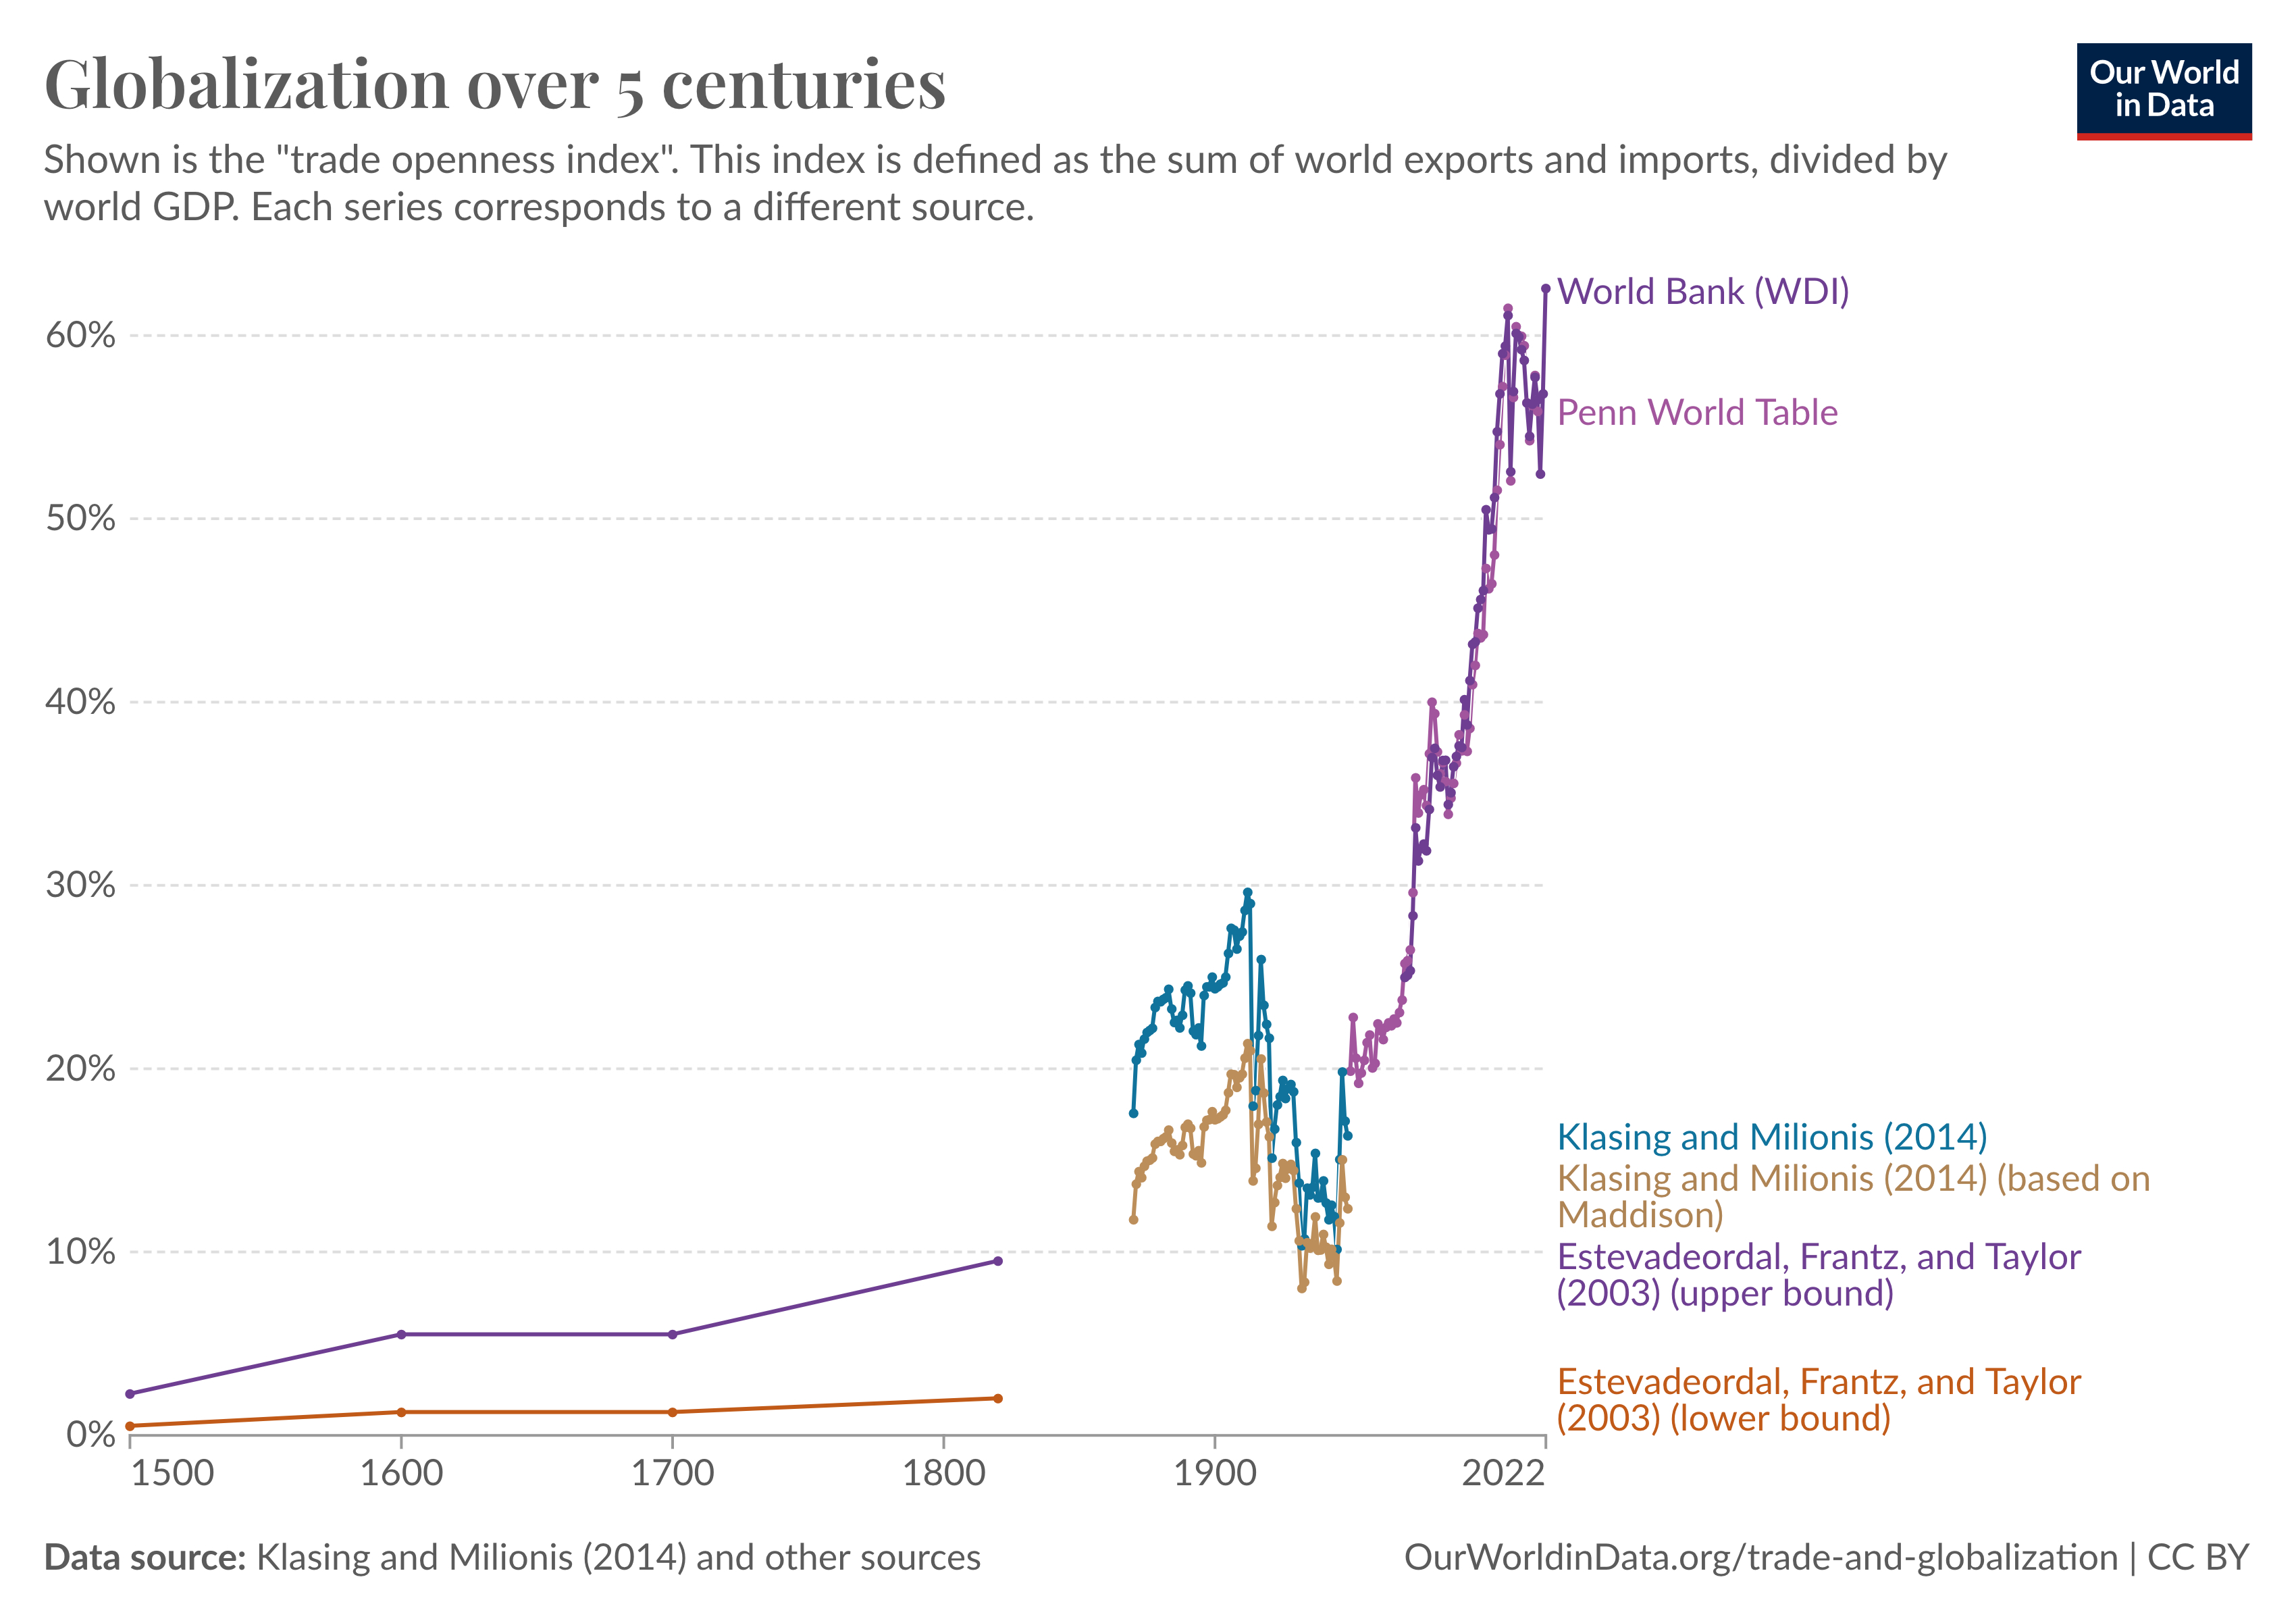
\includegraphics[width=0.9\linewidth]{globalization-over-5-centuries.jpg}
\end{figure}
\end{frame}

\begin{frame}{Direction of Trade}
\begin{figure}
    \centering
    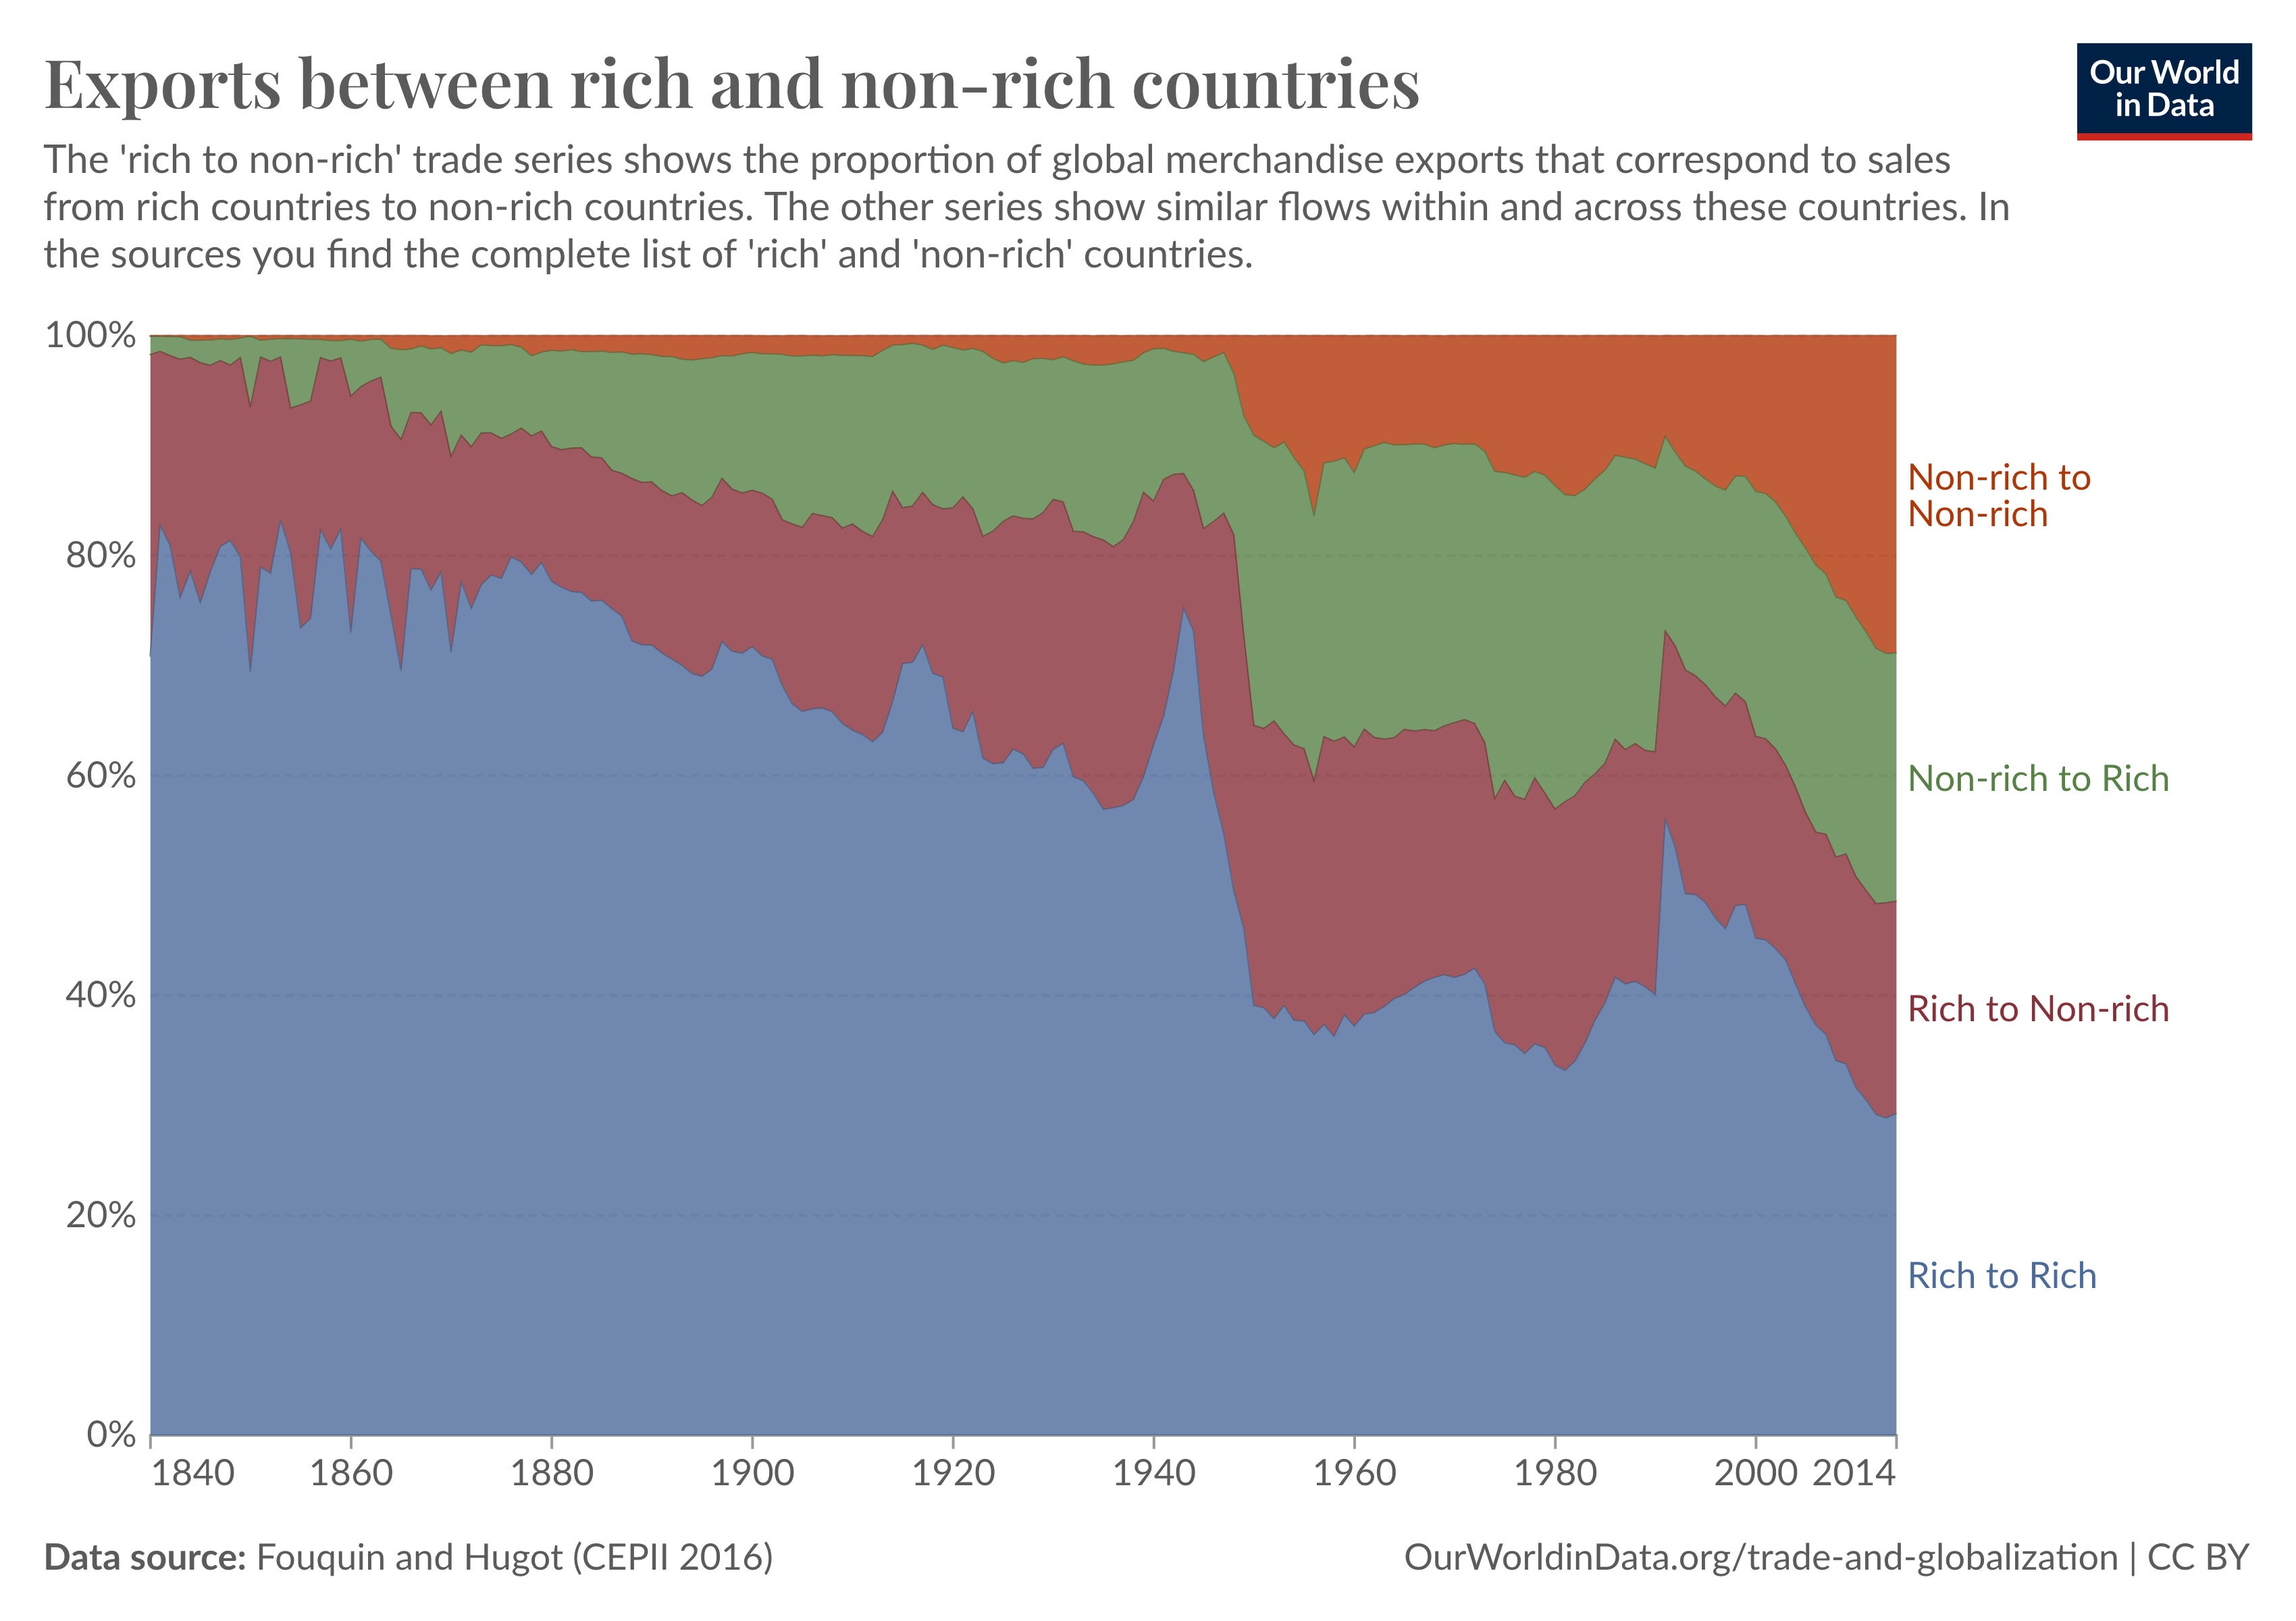
\includegraphics[width=0.9\linewidth]{exports between rich and non-rich countries over time.jpg}
\end{figure}
\end{frame}

\begin{frame}{Costs of Connectedness}
\begin{figure}
    \centering
    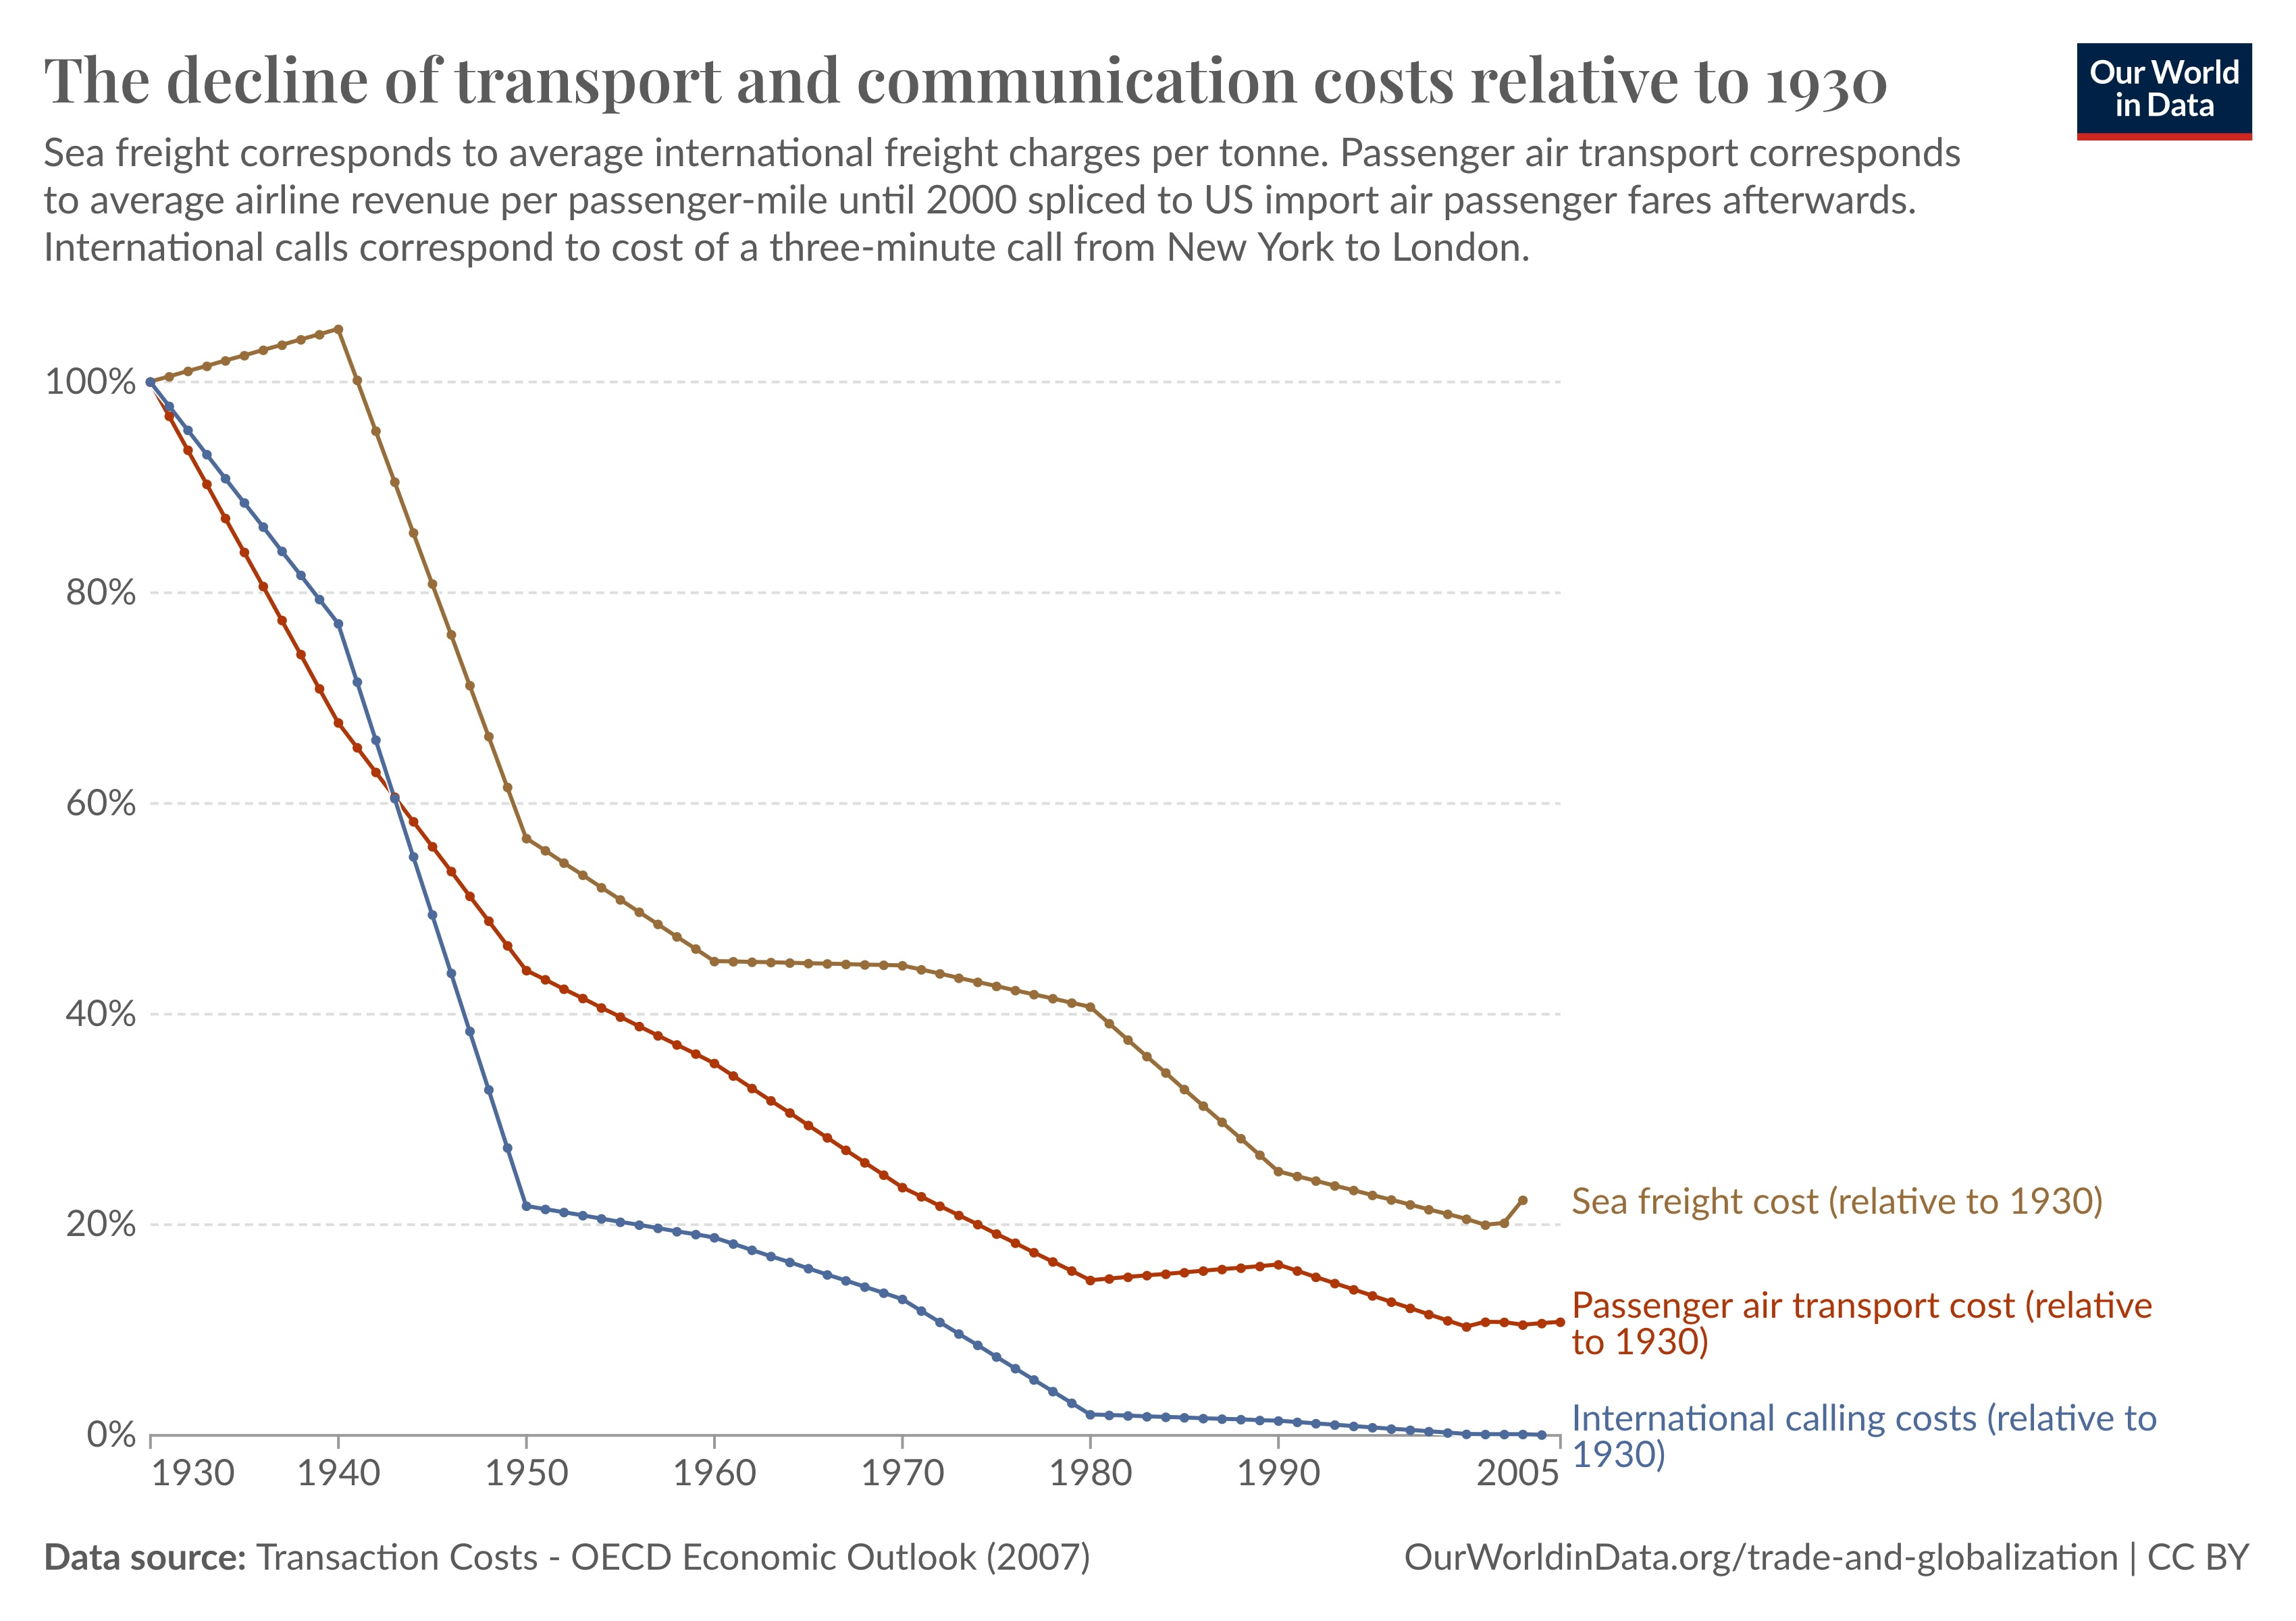
\includegraphics[width=0.9\linewidth]{real-transport-and-communication-costs.jpg}
\end{figure}
\end{frame}

\begin{frame}{Transportation Revolution: The Container}
\small
\begin{columns}
\begin{column}{0.5\textwidth}
    \textbf{Before Containerization:}
    \begin{itemize}
        \item Cargo loaded piece by piece
        \item Loading 5,000 tons: 1 week, 70 workers
        \item Costs dominated by handling, not transport
    \end{itemize}
    \textbf{The Container Revolution :}
    \begin{itemize}
        \item 1956: Standardized metal boxes
        \item Intermodal: ship $\rightarrow$ train $\rightarrow$ truck, seamlessly
        \item Loading 5,000 tons: <8 hours, 5 workers
    \end{itemize}
\end{column}
\begin{column}{0.5\textwidth}
\begin{figure}
    \centering
    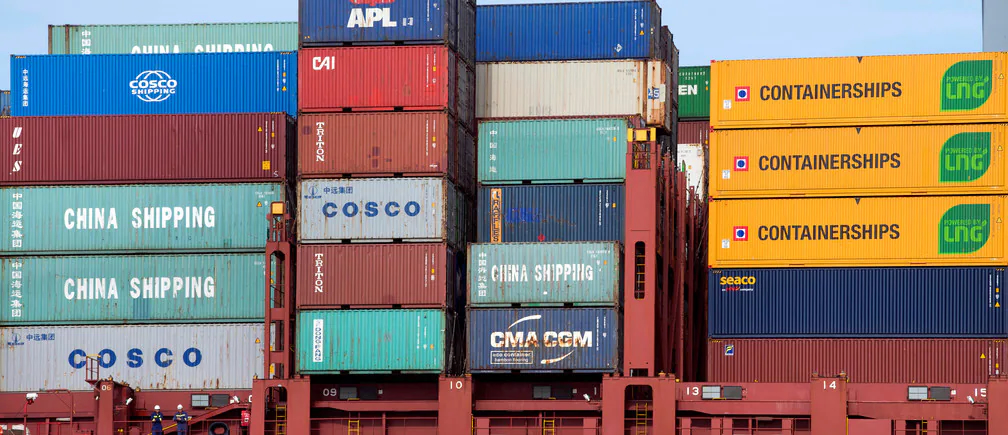
\includegraphics[width=\linewidth]{container.jpeg}
\end{figure}
    \textbf{Economic Impact:}
    \begin{itemize}
        \item Made low-value, high-volume trade profitable
        \item Enabled just-in-time manufacturing
        \item Port cities without space for container yards declined (e.g., New York, San Francisco)
    \end{itemize}
\end{column}
\end{columns}
\end{frame}

\begin{frame}{Communication Revolution: From Telegraph to Internet}

\textbf{Cost Decline Example:} 3-minute call NY-London:
\begin{itemize}
    \item 1930: \$244.65 (in 2010 US dollars)
    \item 1970: \$31.58
    \item 1990: \$3.32
    \item 2020: Effectively \$0 (WhatsApp, Telegram)
\end{itemize}

\end{frame}

\begin{frame}{Tourist Trips}
    \begin{figure}
        \centering
        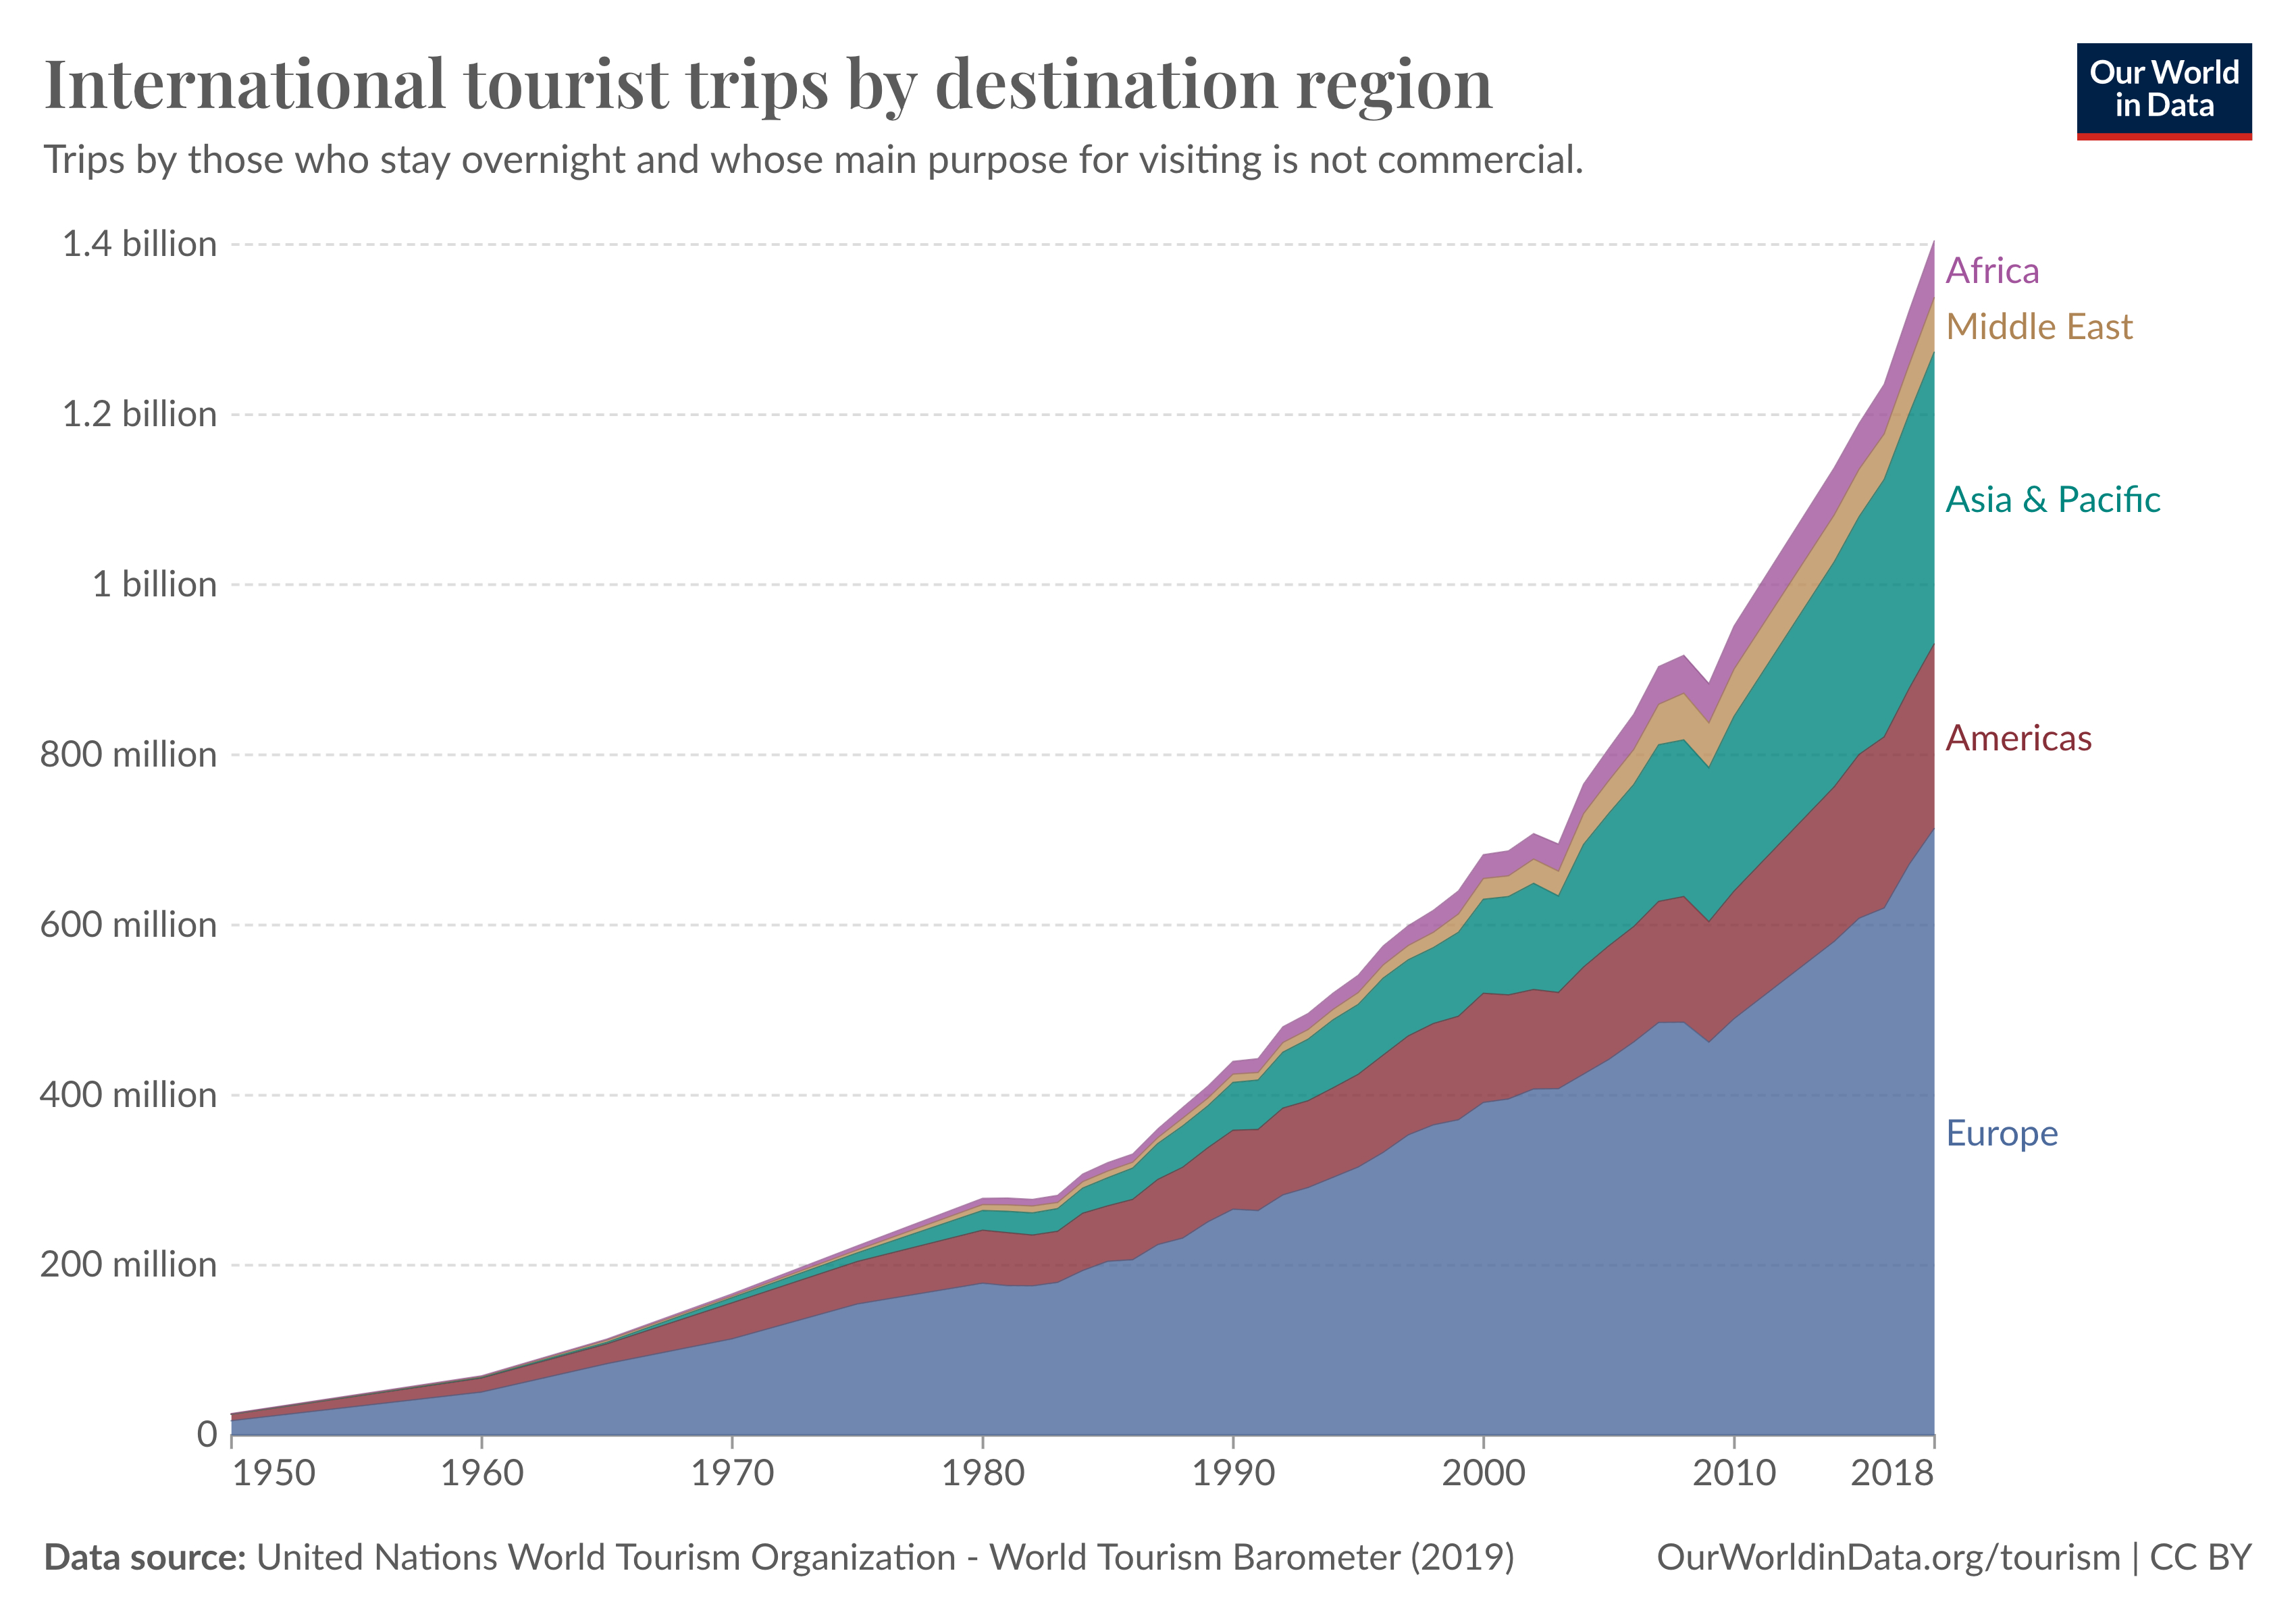
\includegraphics[width=0.9\linewidth]{international-tourist-trips-by-destination-region.jpg}
    \end{figure}
\end{frame}


\section{Historical Background}

\begin{frame}{Early Trade Networks (Before 1500)}
\small
\begin{columns}
\begin{column}{0.5\textwidth}
    \textbf{Pre-Modern Trade Routes:}
    \begin{itemize} \footnotesize % before common era (before year 1 in the Gregorian calender)
        \item \textbf{Silk Road (130 BCE - 1453 CE):} Connected China to Mediterranean through Central Asia. Traded silk, spices, precious metals, ideas, and religions.
        \item \textbf{Indian Ocean Trade:} Maritime trade between East Africa, Arabia, India, and Southeast Asia. Peak period: 800-1500.
        \item \textbf{Trans-Saharan Routes (since 1000 BCE):} Gold, salt, and enslaved people traded across the Sahara. Timbuktu emerged as a major trading centre in the 14th century.
    \end{itemize}
\end{column}
\begin{column}{0.5\textwidth}
    \begin{tcolorbox}[colback=deepblue!5!white,colframe=deepblue!75!black,title=Key Insight]
    Trade has existed for millennia, but was limited by: % and cultural exchange
    \begin{itemize} \small
        \item High transportation costs % before railroads, standardized containers, or motorized vehicles
        \item Limited information flows % how do I know that someone in a different region, speaking a different language is willing to trade something that I desire?
        \item Smaller scale (luxury goods, not mass commodities) % given the transportation costs, it's less likely to trade common produce, like meat (today we can buy meat from south america in european supermarkets. This was not feasible (has to be kept cold the entire time) and furthermore the high costs od transportation don't make it economic to do so)
    \end{itemize}
    \end{tcolorbox}
\end{column}
\end{columns}
%Source: \cite{findlay2007power} - "Power and Plenty: Trade, War, and the World Economy in the Second Millennium"
\end{frame}

\begin{frame}{"The Age of Exploration" (1500-1800)}
\small
    \textbf{The Columbian Exchange:} % the name columbian comes from Christopher Columbus, because his voyage in 1492 marked the beginning of this period of european invasion 
    \begin{table}[h]
    \scriptsize
    \begin{tabular}{p{4cm}|p{4cm}}
    \toprule
    \textbf{Old World → New World} & \textbf{New World → Old World} \\
    \midrule
    Sugar, coffee, soybeans & Maize, potatoes, tomatoes \\
    Smallpox, measles, chickpox & Tobacco, cacao \\
    \bottomrule
    \end{tabular}
    \end{table}
% Columbian Exchange refers to the exchange of diseases, ideas, food, crops, and populations between the New World and the Old Worldcrops, and populations between the New World and the Old World 
% introducing food from the new world to the old world had benefits because of different weather requirements, making them suitable as a complement to existing plants
% In many cases, the Old World crops were grown much more productively in the New World soils and climate
    \textbf{Impact:} Society and population transformed. Potatoes enabled European population growth. Diseases devastated Indigenous Americans (between 80-95\% depopulation in the first 150 years after the European invasion).
  % the potato is dense in nutrients and calories so it is the food most suitable for sustaining a diet solely made up of it  
    \begin{itemize} \small
        \item ''Transatlantic slave trade'': $\approx$ 12.5 million Africans forcibly taken to the Americas (1525-1866)
        \item Mercantilist colonial systems: Forced labor on plantations and trade policies designed to extract raw materials for European benefit while prohibiting colonial manufacturing
        % colonies exist to benefit the mother country, raw materials are extracted using cheap or forced labor, these materials are exclusively sold back to the mother country for cheap prices
        % manufactured (final goods) are exclusively bought from the mother country at high prices -> this aids the mother countries population and economy
        % prohibit colonial manufacturing. If colonies are able to turn their raw materials (cotton) into cloth and fabric themselves, there is no need to import final goods (manufactured goods) from the mother country 
        % This created a deliberate economic dependency: colonies stayed poor and the development of an industrialized economy is prohibited while the mother country industrializes and is growing rich using colonial resources and captive labor markets.
    \end{itemize}
\end{frame}

\begin{frame}{The First Wave (1870-1914): Transportation and Industrialization}
    \begin{itemize}
        \item Triggered by a stark decrease in transportation costs (steam engines, railways), boosted by the Industrial Revolution in Great Britain.
        \item Mass migration from Europe to North America and Australia, as well as from China and India to Sri Lanka, Burma, Thailand, the Philippines, and Vietnam (in total around 10\% of the world's labour force on the move) (\cite{worldbank2005trade}).
        % land in the new world was abundant and the migration from Europe tightened the labour market (workers were more scarce, which raised wages)
        \item Period ended by the first world war, retaliatory tariffs during the Great Depression of the 1930s, and immigration restrictions in the US. 
    \end{itemize}
\end{frame}

\begin{frame}{The Interwar Period (1914-1945): Globalization in Reverse}
\small
\begin{columns}
\begin{column}{0.5\textwidth}
    \textbf{The Collapse of the First Wave:}
    
\begin{figure}
    \centering
    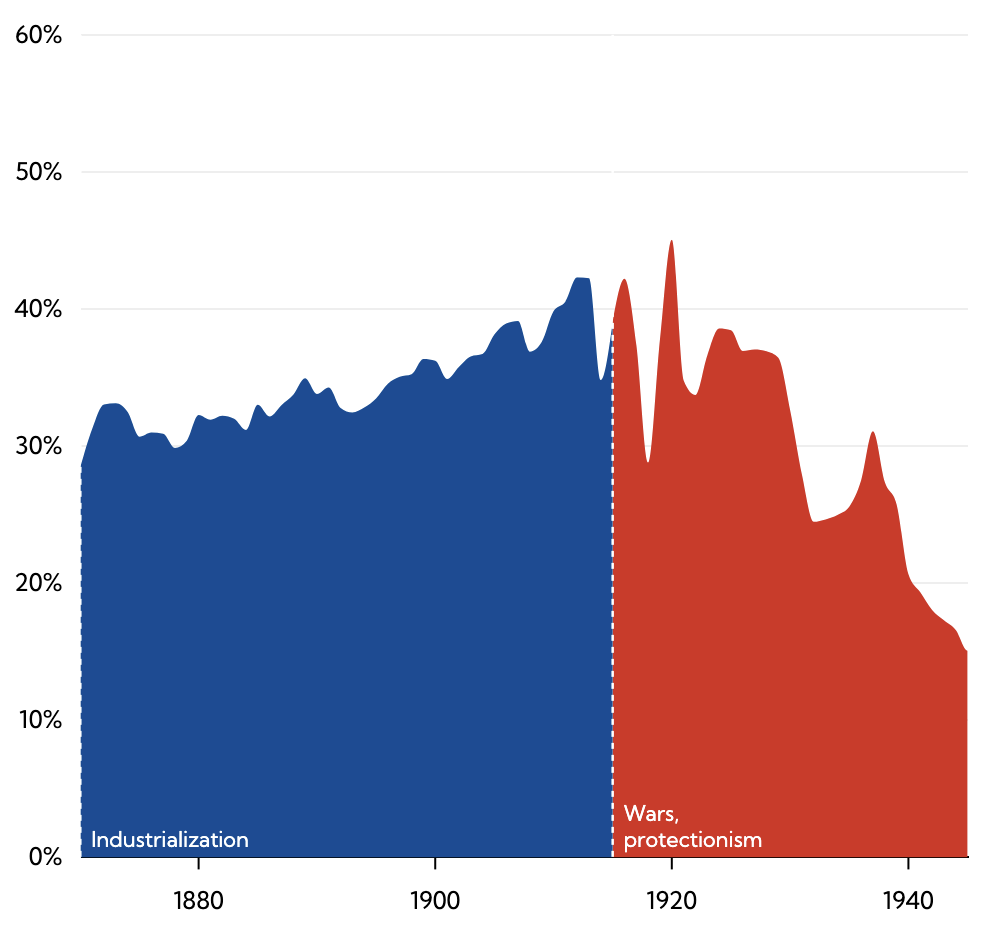
\includegraphics[width=0.8\linewidth]{interwar period.png}
    \caption{Sum of imports and exports as a share of GDP. Source: IMF}
    \label{fig:placeholder}
\end{figure}
\end{column}
\begin{column}{0.5\textwidth}
    \begin{itemize} \footnotesize
        \item \textbf{WWI (1914-18)} 
        \item \textbf{US tariffs of up to 53\% (1930):} 60+ countries retaliated
        \item \textbf{Great Depression:} Global trade fell by 65\% (1929-1932)
        \item \textbf{Immigration restrictions:} US quotas ended open borders
    \end{itemize}
    \begin{tcolorbox}[colback=red!5!white,colframe=red!75!black,title=Warning from History] \footnotesize
    The interwar period shows globalization is \textbf{reversible}. Political choices matter enormously.
    \end{tcolorbox}
\end{column}
\end{columns}
%\vspace{0.2cm}
%\textbf{Poll Question:} Could we see a similar collapse today? What would trigger it?
\end{frame}

\begin{frame}{The Second Wave (1945–80): Policy Liberalization}
\begin{itemize}
    \item Establishment of many international institutions in response to the horrors of nationalism:
\end{itemize}
\vspace{0.2cm} \\
 \begin{minipage}{0.19\textwidth}
        \centering
        
\includegraphics[width=\textwidth]{International_Monetary_Fund_logo.svg.png}
    \end{minipage}
    \begin{minipage}{0.19\textwidth}
        \centering
        
\includegraphics[width=\textwidth]{Flag-United-Nations-Logo.jpg}
    \end{minipage}
    \begin{minipage}{0.19\textwidth}
        \centering
        
\includegraphics[width=\textwidth]{world bank.png}
    \end{minipage}
    \begin{minipage}{0.19\textwidth}
        \centering
        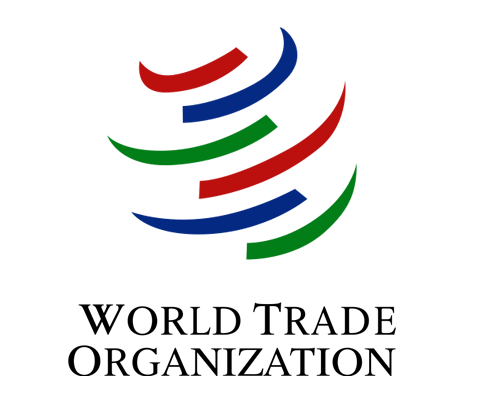
\includegraphics[width=\textwidth]{wto logo.png}
    \end{minipage}
    \begin{minipage}{0.19\textwidth}
        \centering
        
\includegraphics[width=\textwidth]{European Economic Community.png}
    \end{minipage}
\begin{itemize}
    \item Especially in rich countries, this second wave of internationalization led to specialization, clusters of production and sunk costs because of economies of scale.
\end{itemize}    
\end{frame}

%\begin{frame}{GATT and the WTO: Institutionalizing Free Trade}
%\small
%\begin{columns}
%\begin{column}{0.55\textwidth}
 %   \textbf{General Agreement on Tariffs and Trade (1947):}
 %   \vspace{-0.3cm}\\
  %  \begin{table}[h]
   % \scriptsize
    %\begin{tabular}{l|c|p{3cm}}
%    \toprule
 %   \textbf{Round} & \textbf{Years} & \textbf{Achievement} \\
  %  \midrule
   % Geneva & 1947 & Initial 45,000 tariff concessions \\
    %Kennedy & 1964-67 & 35\% tariff cut \\
%    Tokyo & 1973-79 & Non-tariff barriers \\
 %   Uruguay & 1986-94 & Services, IP, created WTO \\
  %  \bottomrule
   % \end{tabular}
    %\end{table}
%\end{column}
%\begin{column}{0.45\textwidth}
 %   \textbf{World Trade Organization (1995):}
  %  \begin{itemize}
   %     \item 164 members (as of 2023)
    %    \item Covers goods, services, intellectual property
     %   \item Average tariff on manufactures: 50\% (1947) $\rightarrow$ 4\% (2000s)
    %\end{itemize}
%\end{column}
%\end{columns}
%\end{frame}

\begin{frame}{Economic Integration}
\textbf{Levels of Economic Integration:}
\begin{enumerate}
    \item \textbf{Free Trade Area:} Remove tariffs (e.g., NAFTA)
    \item \textbf{Customs Union:} + common external tariff (e.g., Turkey-EU)
    \item \textbf{Common Market:} + free movement of factors (labor, capital)
    \item \textbf{Economic Union:} + coordinated policies (e.g., EU)
    \item \textbf{Political Union:} + shared institutions (EU aspiration)
\end{enumerate}
\end{frame}

\begin{frame}{Third Wave (1989-): Financial Integration and Digital Technology}
    Also called the "New Wave of Globalization". \\
    \begin{itemize}
        \item Inclusion of developing countries into international markets.
        \item China's inclusion into the WTO in 2001
        \item Increase in the export of services and a globalization of financial flows thanks to the enabling technology of computers and the internet. % in economics, we define output of an economy (GDP) as the sum of goods and services produced within one year. Goods are final goods meant for final consumption, they are not meant to be refined. Goods can be cars, clothing, fresh produce etc.
        % Services are activities that provide value for the society and the economy without producing a physical good. It's things like getting a haircut, paying someone to clean the apartment, healthcare, hospitality (hotels, restaurants), transportation. While you can't trade services like getting a haircut, certain professional services like accounting, legal advise don't necessarily need to come from within your country of residence, education can take place online, financial services like banking and investment are primarily remote and information and communication services are remote as well  
        \item End of the Cold War and fall of the Iron Curtain in 1991. % followed by increased trade with countries of the former societ union, the east enlargement of the EU, and pick up of diplomatic relations between parties of opposing sites of the Cold War
        \item The financial crisis, the pandemic, and increasing nationalism are possibly moving us towards a time of deglobalization. % Can you explain to me why?
        % Answer: pandemic disclosed economic vulnerabilities from dependency on foreign production, displayed the need to be self-sufficient to a certain degree. "reshore" or "nearshore" manufacturing of critical goods.
        % international cooperation can collapse when nations prioritized self-preservation. Vaccines were horded and distributed among the own population first 
        % Politicians gained support by blaming globalization for job losses and promising to protect domestic industries.
        % who of you has seen the movie the "the big short". It describes how the financial crisis was triggered by the US subprime martgage market of the US. The crisis revealed how interconnected global finance created systemic risk because not only the US was affected, the bank Lehman Borthers failed and this had repercussions for the entire world economy. It triggered a change in ideology from a neoliberal idea of free markets that regulate themselves, towards more state intervention. And there is a connection to nationalism because the financial crisis fueled policies of austerity (government policies that reduce public spending and/or increase taxes to decrease budget deficits and government debt), which created economic hardship for certain groups in society and has been found to fuel nationalistic and populist movements
    \end{itemize}
\end{frame}

\section{Cultural Dimension}
\small
\begin{frame}{Cultural Globalization: Homogenization or Hybridization?}
\begin{columns}
\begin{column}{0.5\textwidth}
    \textbf{Evidence of Cultural Convergence:}
    \begin{itemize}
        \item \textbf{Brands:} McDonald's in 100+ countries; Starbucks, Nike globally visible
        \item \textbf{Media:} Hollywood dominates global box office; Netflix streams worldwide
        \item \textbf{Language:} English as the default language for international communication
        \item \textbf{Beauty standards:} Ideals spread via social media
    \end{itemize}
\end{column}
\pause
\begin{column}{0.5\textwidth}
    \textbf{Counter-Evidence:}
    \begin{itemize}
        \item McDonald's adapts: McAloo Tikki (India), Teriyaki Burger (Japan), Poutine (Canada)
        \item Work cultures persist: siesta remains in Spain despite global business hours pressure
        \item Food practices: many cultures maintain distinct meal timing and eating customs % eating on the go or eating for hours
        \item Religious revivalism and identity politics rising 
    \end{itemize}
\end{column}
\end{columns}
\end{frame}

\begin{frame}{Student Poll}
\large
   Do you think that your generation is more culturally homogeneous than your grandparents' generation? \\ What makes you think so? \\ How would you define cultural lines? \\ Is there such a thing as national culture? \pause \vspace{1cm}\\
   \begin{center}
       \href{https://www.youtube.com/watch?v=LYCKzpXEW6E}{\textcolor{red}{Ted Talk on Sovereign States and Culture}}
   \end{center}
\end{frame}



\end{document}

